% Copyright (c) 2008, João Henrique Ferreira de Freitas
% All rights reserved.
% 
% Redistribution and use in source and binary forms, with or without modification,
% are permitted provided that the following conditions are met:
% 
%     * Redistributions of source code must retain the above copyright notice,
%       this list of conditions and the following disclaimer.
%     * Redistributions in binary form must reproduce the above copyright notice,
%       this list of conditions and the following disclaimer in the documentation and/or 
%       other materials provided with the distribution.
%     * Neither the name of the <ORGANIZATION> nor the names of its contributors may
%       be used to endorse or promote products derived from this software without 
%       specific prior written permission.
% 
% THIS SOFTWARE IS PROVIDED BY THE COPYRIGHT HOLDERS AND CONTRIBUTORS "AS IS" AND ANY 
% EXPRESS OR IMPLIED WARRANTIES, INCLUDING, BUT NOT LIMITED TO, THE IMPLIED WARRANTIES
% OF MERCHANTABILITY AND FITNESS FOR A PARTICULAR PURPOSE ARE DISCLAIMED. IN NO EVENT
% SHALL THE COPYRIGHT OWNER OR CONTRIBUTORS BE LIABLE FOR ANY DIRECT, INDIRECT, INCIDENTAL,
% SPECIAL, EXEMPLARY, OR CONSEQUENTIAL DAMAGES (INCLUDING, BUT NOT LIMITED TO, PROCUREMENT
% OF SUBSTITUTE GOODS OR SERVICES; LOSS OF USE, DATA, OR PROFITS; OR BUSINESS INTERRUPTION)
% HOWEVER CAUSED AND ON ANY THEORY OF LIABILITY, WHETHER IN CONTRACT, STRICT LIABILITY,
% OR TORT (INCLUDING NEGLIGENCE OR OTHERWISE) ARISING IN ANY WAY OUT OF THE USE OF THIS
% SOFTWARE, EVEN IF ADVISED OF THE POSSIBILITY OF SUCH DAMAGE.
% 
% $Id$

\section{Objetivos} \label{sec:objetivos}

% Elaborar um processo formal ou semiformal para usuários de SL/CA que futuramente necessitem contribuir com um projeto enviando patchs, melhoramentos e contribuições. O trabalho prevé o entendimento da lógica de colaboração utilizada em alguns projetos explanados durante o tema.

Este trabrabalho tem como objetivo primordial estudar o ciclo de desenvolvimento, mais especificadamente sobre o processso de contribuição, utilizado em um projeto de SL/CA previamente escolhido. A fim de observar e coletar dados acerca da colaboração entre desenvolvedores do núcleo do projeto e desenvolvedores periféricos ou usuários com necessidades específicas ainda não contempladas pelo projeto.

Entende-se, neste contexto, por colaboração o envio de patchs \cite{preliminary} que são definidos como mudanças, consertos ou melhoramentos e podem conter por exemplo trechos de código fonte, melhoria de documentação, e em última instância melhoria da engenharia de software.

% Não é o foco do trabalho estudar e criar um processo para ser utilizado como guias gerais mas sim demonstrar como um usuário desenvolvedor pode adicionar recursos ao software, utilizando para isso técnicas de engenharia de software e áreas coligadas.


Como definido em \cite{introducaoslca} \textit{``Projeto de Software Livre é uma organização virtual, com nome próprio, centrada em torno de um código fonte, com participação espontânea e variável de usuários e desenvolvedores... implementando um processo de software individualmente determinado''}. Assim definimos o termo ``Projeto de SL/CA'' neste trabalho. 

Também esclarecemos a posição usada para a coleta de dados e evidenciação. De acordo com a figura \ref{fig:equipe}, representando a forma de organização dos individuos na comunidade, nós nos situamos entre \textit{usuários}, \textit{desenvolvedores esporádicos} e \textit{desenvolvedores frequentes} podendo assim capturar as interações necessárias. 

Ao passo da pesquisa, identificamos algumas questões as quais ajudaram a salientar a importância do trabalho:

\textit{\begin{itemize}
 \item Como colaborar efetivamente?
 \item Quais os caminhos e possibilidades para usuários de qualquer projeto de SL/CA podem utilizar para desenvolvever e integrar patchs nos projetos?
 \item Como planejar os melhoramentos e qual a melhor forma de planejá-los?
 \item Como validar e eliciar os requisitos de melhoramento?
 \item Quais os recursos que o desenvolvedor tem para verificar os requisitos de melhoramento?
 \item Como atrair atenção para o seu trabalho?
 \item Como não gerar retrabalho e quais os meios e ferramentas necessários?
 \item Como submeter a contribuição?
 \item Como avaliar resultados obtidos?
\end{itemize}}


\begin{figure}
 \centering
 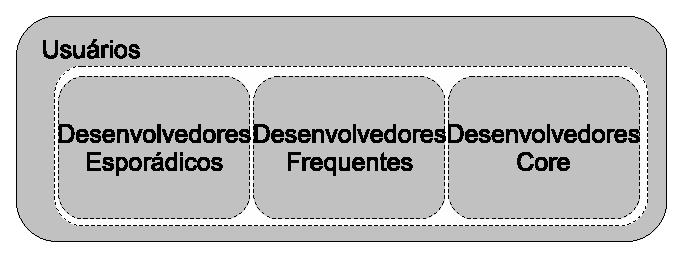
\includegraphics{../../doc/diagramas/equipe.eps}
 % equipe.eps: 1179666x1179666 pixel, 300dpi, 9987.84x9987.84 cm, bb=0 0 482 213
 \caption[Equipe numa comunidade virtual]{Diagrama representando a equipe numa comunidade virtual \cite{introducaoslca}}
 \label{fig:equipe}
\end{figure}
